\chapter{概率论的基本概念}
自然界中发生的现象是多种多样的,有这样一类现象,在一定条件下必然会发生,例如,向上抛一物体必然下落,同性电荷必然相互排斥,异性电荷必然相互吸引,等等,这类现象称为\uwave{确定性现象}(Deterministic Phenomenon)。但是,还有这样一类现象,例如,在相同条件下抛同一枚硬币,其落下后,可能朝上,可能朝下。这里现象,在一定的条件下,可能出现这样的结果,可能出现那样的结果,但是经过长期实践并深入研究后,发现这类现象在大量重复试验或观察下,它的结果却呈现出某种规律性,抛硬币得到正面朝上和反面朝上的情况数大概都是一半。这种在大量重复试验或观察中所呈现出的固有规律性,就是我们之后所说的\uwave{统计规律性}(Statistical Regularity)。综上,\empx{在个别试验中结果呈现出不确定性,在大量重复试验中结果又具有统计规律性的现象},我们称之为\uwave{随机现象}(Random Phenomenon)。而所谓\uwave{概率论}(Probability Theory)与\uwave{数理统计}(Mathematical Statistics),即研究统计规律的数学。

\section{随机试验}
我们遇到过各种试验,在这里,我们把试验作为一个含义广泛的术语,例如
\begin{itemize}
    \item $E_1$:将一枚硬币抛掷一次,观察正面$H$和反面$T$出现的情况。
    \item $E_2$:将一枚硬币抛掷三次,观察正面$H$和反面$T$出现的情况。 
    \item $E_3$:抛一颗骰子,观察出现的点数。
    \item $E_4$:在一批灯泡中任意抽取一只,测试它的极限寿命(以小时为单位)。
\end{itemize}
我们这里举了四个试验的例子,它们有一些共同的特点,我们总结如下
\begin{BoxDefinition}[随机试验]
    \uwave{随机试验}(Experiment)是指具有下述三个特点的试验,常记为$E$
    \begin{enumerate}
        \item 可以在相同的条件下重复进行。
        \item 试验的可能结果不止一个,并且事先能明确试验的所有可能结果。
        \item 试验进行之前,我们无法确定哪一个结果会出现
    \end{enumerate}
\end{BoxDefinition}


\section{随机事件与样本空间}

\subsection{样本空间和样本点}
关于\fancyref{def:随机试验}中提到的一个随机试验,尽管在每次试验前并不能预知试验的结果,但试验的所有可能组成的集合是已知的,这种集合,可以是有限集,可以是无限集。
\begin{BoxDefinition}[样本空间]
    定义随机试验$E$每个可能的结果组成的集合$S$,为$E$的\uwave{样本空间}(Sample Space)
    \begin{Equation}
        S=\qty{e_1,e_2,\cdots,e_i,\cdots}
    \end{Equation}
\end{BoxDefinition}
\begin{BoxDefinition}[样本点]
    定义随机试验$E$的每个结果$e_i$,为$E$的\uwave{样本点}(Sample Point)。
\end{BoxDefinition}

例如\xref{sec:随机试验}中列出的试验$E_1,E_2,E_2,E_3$的样本空间就是
\begin{Gather}*[6pt]
    S_1:\qty{H,T}\\
    S_2:\qty{HHH,HHT,HTH,HTT,THH,THT,TTH,TTT}\\
    S_3:\qty{1,2,3,4,5,6}\\
    S_4:\qty{t\mid t\geq 0}
\end{Gather}
而上述样本空间的集合中的每个元素,就是样本点。

\subsection{随机事件}
在实际中,当进行随机试验时,我们常常关心某些样本点所组成的集合。
\begin{BoxDefinition}[随机事件]
    \uwave{随机事件}(Event)是随机试验$E$的样本空间$S$的一个子集,常记为$A$

    在每次试验$E$中,当且仅当该子集$A$中一个样本点发生,我们称这一事件$A$发生。
\end{BoxDefinition}

例如,关于\xref{sec:随机试验}中掷骰子的随机试验$E_3$
\begin{itemize}
    \item 事件$A_1$是掷出点数$2$,则$A_1=\qty{2}$
    \item 事件$A_2$是掷出偶数点数,则$A_2=\qty{2,4,6}$
\end{itemize}
特别的,我们赋予那些仅包含一个样本点的事件一个特别的名称,即基本事件。
\begin{BoxDefinition}[基本事件]
    \uwave{基本事件}(Elementary Event)是指仅包含一个样本点的事件。
\end{BoxDefinition}
\begin{itemize}
    \item 掷骰子的试验$E_3$中,基本事件有六个,有$\qty{1},\qty{2},\qty{3},\qty{4},\qty{5},\qty{6}$
    \item 掷硬币的试验$E_1$中,基本事件有两个,有$\qty{H},\qty{T}$
\end{itemize}

% 除此之外,还有两个特别的事件需要定义
\begin{BoxDefinition}[必然事件]
    定义\uwave{必然事件}(Certain Event)为样本空间$S$自身,它是$S$的子集。
\end{BoxDefinition}
\begin{BoxDefinition}[不可能事件]
    定义\uwave{不可能事件}(Impossible Event)为空集$\empty$,它是$S$的子集。
\end{BoxDefinition}

\subsection{随机事件的关系与运算}
我们说,\empx{事件是一个集合},因此,事件间的关系和运算可以按照集合论中集合之间的关系和运算来处理,下面,我们将根据“事件发生”的含义,给出这些运算在概率论中的具体含义。

\begin{BoxDefinition}[事件的包含]
    若$A\subset B$,则称事件$B$包含事件$A$,即事件$A$发生必然导致事件$B$发生。
\end{BoxDefinition}

\begin{BoxDefinition}[事件的相等]
    若$A\subset B$又有$B\subset A$,则称事件$B$等于事件$A$,记为$A=B$。
\end{BoxDefinition}

\begin{BoxDefinition}[和事件]
    定义$A,B$的\uwave{和事件}(Union of Events)
    \begin{Equation}
        A\cup B=\qty{x\mid x\in A~\text{or}~x\in B}
    \end{Equation}
    其意义是,当且仅当$A,B$至少有一个发生时,和事件$A\cap B$发生。
\end{BoxDefinition}

\begin{BoxDefinition}[积事件]*
    定义$A,B$的\uwave{积事件}(Intersection of Events)
    \begin{Equation}
        A\cap B=AB=\qty{x\mid x\in A~\text{and}~x\in B}
    \end{Equation}
    其意义是,当且仅当$A,B$同时发生时,积事件$A\cup B$发生。
\end{BoxDefinition}

\begin{BoxDefinition}[差事件]
    定义$A,B$的\uwave{差事件}(Set Difference)
    \begin{Equation}
        A-B=\qty{x\mid x\in A~\text{and}~x\notin B}
    \end{Equation}
    其意义是,当且仅当$A$发生且$B$不发生,差事件$A-B$发生。
\end{BoxDefinition}

\begin{BoxDefinition}[互斥事件]
    若事件$A.B$满足下式,则$A,B$是\uwave{互斥}的
    \begin{Equation}
        A\cap B=\empty
    \end{Equation}
\end{BoxDefinition}

\begin{BoxDefinition}[对立事件]
    若事件$A.B$满足下式,则$A,B$是\uwave{对立}的
    \begin{Equation}
        A\cap B=\empty\qquad A\cup B=S
    \end{Equation}
\end{BoxDefinition}
很明显,对立事件是互斥事件的一种特殊情况,对立必然互斥,但对立还要求“除了$A,B$没有更多情况”,因此,我们可以将$A$唯一的那个对立事件记为$\bar{A}$,显然其满足$\bar{A}=S-A$。

\section{频率与概率}
对于一个事件来说,它在一次试验中可能会发生,也可能不会发生。我们常常希望知道某些事件在一次试验中发生的可能性有多大,我们希望找到一个合适的数来表征可能性的大小。为此,首先引入频率,它描述了事件发生的频繁程度,进而引出表征可能性大小的数,即概率。

\subsection{频率}
\begin{BoxDefinition}[频率]*
    在相同条件下,进行$n$次试验,记$n_A$为其中事件$A$发生的次数。

    定义$n_A$为$A$的\uwave{频数}(Frequency),定义$A$的\uwave{频率}(Relative Frequency)为\footnote[2]{需要注意,虽然物理上frequency就是频率,但统计上frequency是指频数。}
    \begin{Equation}
        f_n(A)=\frac{n_\text{A}}{n}
    \end{Equation}
    其中$f_n(A)$代表的是$A$在进行$n$次试验时的频数。
\end{BoxDefinition}\goodbreak

很容易验证,频率应具有以下的性质
\begin{BoxProperty}[频率的性质]
    频率具有以下基本性质
    \begin{enumerate}
        \item 频率总是在$0$和$1$间,即$0\leq f_n(A)\leq 1$
        \item 频率对于必然事件而言总是$1$,即$f_n(S)=1$
        \item 若$A_1,A_2,\cdots,A_n$是两两不相容的事件,则
        \begin{Equation}
            f_n(A_1\cup A_2\cup\cdots\cup A_n)=f_n(A_1)+f_n(A_2)+\cdots +f_n(A_n)
        \end{Equation}
    \end{enumerate}
\end{BoxProperty}

频率越大,事件发生的越频繁。但是,频率对于一个试验来说并不是一个唯一的值,进行的试验次数$n$不同,或者进行试验次数$n$相同的两组试验,得到的频率可能都是不同的,因此用频率表示可能性是不合适的。然而大量试验证实,当重复试验的次数$n$逐渐增大趋于无穷大时,频率$f_n(A)$呈现出稳定性,逐渐稳定于某个常数。这种频率稳定性即通常所说的统计规律性,让试验重复大量次数,计算频率$f_n(A)$,以它表征事件$A$发生的可能性是非常合适的。

然而在实际中,我们不可能对每一个事件都做大量的试验,因此,为了理论研究的需要,我们从频率的稳定性和频率和性质出发,给出如下表征事件发生可能性大小的概率的定义。

\subsection{概率}
\begin{BoxDefinition}[概率]
    若对于随机试验$E$的每一事件$A$赋予一个实数$P(A)$,且集合函数$P(\cdot)$满足
    \begin{enumerate}
        \item \textbf{非负性}:对于每一个事件$A$,有$P(A)\geq 0$
        \item \textbf{规范性}:对于必然事件$S$,有$P(S)=1$
        \item \textbf{可列可加性}:设$A_1,A_2,\cdots$是两两互不相容的事件,则
        \begin{Equation}
            P\qty(\BigCup[k=1][\infty]A_k)=\Sum[k=1][\infty]P(A_k)
        \end{Equation}
    \end{enumerate}
    那么我们就将$P(A)$称为$A$的\uwave{概率}(Probability)。
\end{BoxDefinition}

\xref{def:概率}是概率的公理化定义,称为\uwave{柯尔莫果洛夫公理}(Kolmogorov Axioms)\cite{W1,W2},它非常正确,但确实没有给出更多概率的内涵,我们看不出这和可能性有任何关系。例如对于掷硬币这个事件,直观上应有$P(H)=0.5, P(T)=0.5$,但即便指定$P(H)=0.3, P(T)=0.7$,这也是完全符合概率的公理化定义的,那,岂不是乱套了!这里我们应当指出,\empx{概率和概率律是两件事情},概率的公理化定义只保证概率的取值满足一些最基本的要求,比如硬币抛到正面的概率不能是$3.14$或$-273.15$,而至于说,概率具体是如何分布的,这其实是概率律的问题。\goodbreak

概率律的确立有很多方法,我们上述认为硬币抛出正反面的概率“显然”各为一半,其实就是在通过经验和统计数据建立概率论,而之后,我们还会学习如何通过严格的概率模型去建立概率律\cite{B2}。而结合严格的概率模型之后,我们就可以明确的证明概率是频率在试验次数趋于无穷大的极限(即所谓大数定律),从而确立概率表示可能性的内涵,暂且,先接受这一点。

概率的公理化定理的要求是最低的,例如,它事实上甚至都没有要求概率不能超过$1$,这是因为作为公理,要求总是应该越简单越好,这些很显然的性质其实可以通过三条公理演绎而来。

\begin{BoxProperty}[不可能事件的概率]
    不可能事件的概率为零
    \begin{Equation}
        P(\empty)=0
    \end{Equation}
\end{BoxProperty}

\begin{Proof}
    令$A_k=\empty, k=1,2,\cdots$,则显然
    \begin{Equation}
        \BigCup[k=1][\infty]A_k=\empty
    \end{Equation}
    且对于$\forall i,j\in\N^{*}$,若$i\neq j$,有$A_iA_j=\empty$,因此事件$A_k$之间两两相互独立。

    这样一来,根据\fancyref{def:概率}中概率的可列可加性
    \begin{Equation}
        P(\empty)=P\qty(\BigCup[k=1][\infty]A_k)=\Sum[k=1][\infty]P(A_k)=\Sum[k=1][\infty]P(\empty)
    \end{Equation}
    这就表明$P(\empty)$是无穷多个自身的和,根据\fancyref{def:概率}中概率的非负性,这里又应当有$P(\empty)\geq 0$,为了使上式成立,就必有$P(\empty)=0$,这就证明了不可能事件概率为零。
\end{Proof}

概率的有限可加性的实质,是将概率公理中的可列可加性,限制到有限个的结果。

\begin{BoxProperty}[概率的有限可加性]
    概率的有限可加性是指,若$A_1,A_2,\cdots,A_n$是两两互不相容的事件,则
    \begin{Equation}
        P\qty(\BigCup[k=1][n]A_k)=\Sum[k=1][n]P(A_k)
    \end{Equation}
\end{BoxProperty}



\begin{Proof}
    在$A_1,A_2,\cdots,A_n$的基础上,令$A_{n+1}=A_{n+2}=\cdots=\empty$,显然,
    \begin{Equation}
        \BigCup[k=1][\infty]A_k=
        \BigCup[k=1][n]A_k
    \end{Equation}
    现在$A_k$仍然满足两两互不相容,因此,可以利用\fancyref{def:概率}中概率的可列可加性
    \begin{Equation}
        P\qty(\BigCup[k=1][n]A_k)=
        P\qty(\BigCup[k=1][\infty]A_k)=
        \Sum[k=1][\infty]P(A_k)=\Sum[k=1][n]P(A_k)
    \end{Equation}
    这里最后一步应用了\fancyref{ppt:不可能事件的概率}的$P(\empty)=0$的结论。
\end{Proof}

\begin{BoxProperty}[包含事件的概率]
    设$A,B$是两个事件,若$A\subset B$,则有
    \begin{Equation}
        P(B-A)=P(B)-P(A)
    \end{Equation}
    并且
    \begin{Equation}
        P(B)>P(A)
    \end{Equation}
\end{BoxProperty}

\begin{Proof}
    运用文氏图很容易想象,如果$A\subset B$,那么
    \begin{Equation}
        B=A\cup (B-A)
    \end{Equation}
    并且$A$与$(B-A)$还是互斥的
    \begin{Equation}
        A(B-A)=\empty
    \end{Equation}
    这样就可以应用\fancyref{ppt:概率的有限可加性}
    \begin{Equation}
        P(B)=P(A)+P(B-A)
    \end{Equation}
    移项即得
    \begin{Equation}
        P(B-A)=P(B)-P(A)
    \end{Equation}
    根据\fancyref{def:概率}中概率的非负性,此处$P(B-A)>0$,故$P(B)>P(A)$。
\end{Proof}

\begin{BoxProperty}[概率的上限]
    对于任一事件$A$,总有
    \begin{Equation}
        P(A)\leq 1
    \end{Equation}
\end{BoxProperty}

\begin{Proof}
    由于$A\subset S$,根据\fancyref{ppt:包含事件的概率}和\fancyref{def:概率}的规范性
    \begin{Equation}*
        P(A)\leq P(S)=1\qedhere
    \end{Equation}
\end{Proof}

\begin{BoxProperty}[概率的加法公式]
    对于任意两事件$A,B$,总有
    \begin{Equation}
        P(A\cup B)=P(A)+P(B)-P(AB)
    \end{Equation}
\end{BoxProperty}

\begin{Proof}
    运用文氏图很容易想象,总有
    \begin{Equation}
        A\cup B=A\cup(B-AB)
    \end{Equation}
    并且$A$与$(B-A)$还是互斥的
    \begin{Equation}
        A(B-AB)=\empty
    \end{Equation}
    这样就可以应用\fancyref{ppt:概率的有限可加性}
    \begin{Equation}
        P(A\cup B)=P(A)+P(B-AB)
    \end{Equation}
    这里再应用\fancyref{ppt:包含事件的概率},考虑到$AB\subset B$
    \begin{Equation}*
        P(A\cup B)=P(A)+P(B)-P(AB)\qedhere
    \end{Equation}
\end{Proof}

\begin{BoxProperty}[逆事件的概率]
    对于任一事件$A$,总有
    \begin{Equation}
        P(\bar{A})=1-P(A)
    \end{Equation}
\end{BoxProperty}

\begin{Proof}
    根据\fancyref{def:对立事件},事件$A$和逆事件$\bar{A}$间满足
    \begin{Equation}
        A\cup\bar{A}=S\qquad
        A\bar{A}=\empty
    \end{Equation}
    即$A,\bar{A}$互不相容,故可运用\fancyref{def:可列可加性}
    \begin{Equation}
        P(S)=P(A\cup\bar{A})=P(A)+P(\bar{A})
    \end{Equation}
    而另外一方面,根据\fancyref{def:概率}中概率的规范性
    \begin{Equation}
        P(S)=1
    \end{Equation}
    因此
    \begin{Equation}*
        P(A)+P(\bar{A})=P(S)\qedhere
    \end{Equation}
\end{Proof}
\section{古典概型}
古典概型是概率论发展初期的主要研究对象,它的一些概念直观简单,具有广泛应用。

\subsection{古典概型的定义}
\begin{BoxDefinition}[古典概型]
    若随机试验$E$满足以下两个特征
    \begin{enumerate}
        \item 试验的样本空间仅包含有限个元素。
        \item 试验中的每个基本事件发生的可能性相同。
    \end{enumerate}
    则将随机试验$E$称为\uwave{古典概型}(Classical Probability)或\uwave{等可能概型}。
\end{BoxDefinition}

\subsection{古典概型的概率公式}
\begin{BoxFormula}[古典概型的概率公式]
    若事件$A$包含$k$个基本事件,而样本空间的大小为$n$,则
    \begin{Equation}
        P(A)=\frac{k}{n}
    \end{Equation}
\end{BoxFormula}
\begin{Proof}
    设试验的样本空间为$S=\qty{e_1,e_2,\cdots,e_n}$,根据\fancyref{def:古典概型}
    \begin{Equation}&[1]
        P(\qty{e_1})=
        P(\qty{e_2})=
        \cdots
        P(\qty{e_n})
    \end{Equation}
    由于基本事件是两两互不相容的,且$S=\qty{e_1}\cup\qty{e_2}\cup\cdots\cup\qty{e_n}$
    \begin{Equation}&[2]
        1=P(S)=P\qty(\BigCup[i=1][n]\qty{e_i})=\Sum[i=1][n]P(\qty{e_i})
    \end{Equation}
    将\xrefpeq{1}代入\xrefpeq{2},这里$i$可以是任意小于等于$n$的正整数
    \begin{Equation}&[3]
        1=nP(\qty{e_i})
    \end{Equation}
    故
    \begin{Equation}
        P(\qty{e_i})=\frac{1}{n}
    \end{Equation}
    而事件$A$中包含$k$个基本试验,即$A=\qty{e_{a1},e_{a2},\cdots,e_{ak}}$
    \begin{Equation}*
        P(A)=\Sum[i=1][k]P(\qty{e_{ai}})=\Sum[i=1][k]\frac{1}{n}=\frac{k}{n}\qedhere
    \end{Equation}
\end{Proof}
\section{条件概率}
我们说,假如有100人进行抽签,比如说有2个签或之类的,虽然我们知道,先抽和后抽中签的概率并没有差异,均是$1/100$,但是在等待抽签的过程中,总有这样朴素的想法
\begin{itemize}
    \item 如果上来就有人抽到了签,那么之后我再中签的概率就小很多
    \item 如果上来很多人都没有抽到前,那么之后我再中签的概率就大很多
\end{itemize}
这种朴素的想法,在概率论中称为\uwave{条件概率}。

\subsection{条件概率的定义}
\begin{BoxDefinition}[条件概率]
    设$A,B$是两个事件,且$P(A)>0$,那么将
    \begin{Equation}
        P(B\mid A)=\frac{P(AB)}{P(A)}
    \end{Equation}
    称为在事件$A$发生的条件下,事件$B$发生的\uwave{条件概率}(Conditional Probability)。
\end{BoxDefinition}

事件$B$在事件$A$发生的前提下发生的条件概率为
\begin{Equation}
    P(B\mid A)=\frac{P(AB)}{P(A)}
\end{Equation}
事件$B$发生的概率,其实可以认为是在必然事件$S$发生的前提下发生的条件概率
\begin{Equation}
    P(B)=P(B\mid S)=\frac{P(SB)}{P(S)}
\end{Equation}
条件概率在文氏图中的表示常常是一个挺让人困惑的问题,因为$P(AB)$和$P(B\mid A)$分别代表“$A,B$同时发生的概率”和“$A$发生后$B$发生的概率”,在文氏图上好像都应用$A,B$的交集来表示,但很明显两者又不相等,这怎么解释呢?其实关键在于,样本空间的划定范围,同样是$A,B$的交集,计算$P(AB)$时的样本空间是$S$,计算$P(B\mid A)$时的样本空间则是$A$。

条件概率$P(\cdot\mid A)$,容易验证,亦满足\fancyref{def:概率}的三条概率公理。

\subsection{条件概率与乘法公式}
概率乘法公式,即求两个事件同时发生的概率,其实是\fancyref{def:条件概率}的简单改写。
\begin{BoxFormula}[概率的乘法公式]
    设$A,B$是两个事件,两者同时发生的概率为
    \begin{Equation}
        P(AB)=P(B\mid A)P(A)
    \end{Equation}
\end{BoxFormula}
概率乘法公式是容易理解的,$A,B$同时发生的概率,即$A$发生的概率乘以$A$发生时$B$发生的概率。这种想法也可以很容易的推广到$n$个事件的情形,若有$A_1,A_2,\cdots,A_n$共$n$个事件
\begin{Equation}
    \qquad\quad
    P(A_1A_2\cdots A_n)=P(A_n\mid A_1A_2\cdots A_{n-1})\cdots P(A_3\mid A_2A_1)P(A_2\mid A_1)P(A_1)
    \qquad\quad
\end{Equation}

\subsection{全概率公式和贝叶斯公式}
在介绍全概率公式和贝叶斯公式前,我们先来介绍样本空间的划分的定义。

\begin{BoxDefinition}[划分]
    设$S$为试验$E$的样本空间,$B_1,B_2,\cdots,B_n$为$E$的一组事件,若
    \begin{enumerate}
        \item $B_iB_j=\empty, i,j=1,2,\cdots, n, i\neq j$,即$B_1,B_2,\cdots,B_n$两两互不相容
        \item $B_1\cup B_2\cup\cdots\cup B_n=S$
    \end{enumerate}
    则称$B_1,B_2,\cdots,B_n$是样本空间的一个\uwave{划分}(Partition)。
\end{BoxDefinition}

简而言之,\empx{划分就是将一个集合拆成若干个完备但互不重叠的集合}。

\begin{BoxTheorem}[全概率定理]
    设$A$为$E$的事件,而$B_1,B_2,\cdots,B_n$为$S$的一个划分,且$P(B_i)>0$,则
    \begin{Equation}
        P(A)=\Sum[k=1][n]P(A\mid B_k)P(B_k)
    \end{Equation}
    该结论称为\uwave{全概率定理}(Law of Total Probability)。
\end{BoxTheorem}

\begin{Proof}
    根据\fancyref{def:划分}
    \begin{Equation}&[1]
        A=AS=A(B_1\cup B_2\cup\cdots\cup B_n)
    \end{Equation}
    运用交集(即乘法)对并集的分配律
    \begin{Equation}&[2]
        A=AB_1\cup AB_2\cup\cdots\cup AB_n
    \end{Equation}
    根据\fancyref{def:划分},我们知道$B_1,B_2,\cdots,B_n$两两互不相容,故$AB_1,AB_2,\cdots,AB_n$亦两两互不相容,因此,运用\xrefpeq{2}和\fancyref{ppt:概率的有限可加性},概率$P(A)$可以表示为
    \begin{Equation}&[3]
        P(A)=
        P\qty(\BigCup[k=1][n]AB_k)=\Sum[k=1][n]P(AB_k)
    \end{Equation}
    根据\fancyref{fml:概率的乘法公式}
    \begin{Equation}*
        P(A)=\Sum[k=1][n]P(A\mid B_k)P(B_k)\qedhere
    \end{Equation}
\end{Proof}

\begin{BoxTheorem}[贝叶斯定理]
    设$A$为$E$的事件,而$B_1,B_2,\cdots,B_n$为$S$的一个划分,且$P(A),P(B_i)>0$,则
    \begin{Equation}
        P(B_i\mid A)=\frac{P(A\mid B_i)P(B_i)}{P(A)}=\frac{P(A\mid B_i)P(B_i)}{\Sum[k=1][n]P(A\mid B_k)P(B_k)}
    \end{Equation}
    该结论称为\uwave{贝叶斯定理}(Bayes' Theorem)。
\end{BoxTheorem}
\begin{Proof}
    根据\fancyref{def:条件概率}
    \begin{Equation}
        P(B_i\mid A)=\frac{P(AB_i)}{P(A)}
    \end{Equation}
    在上式中,就$P(A)$代入\fancyref{thm:全概率定理},并使用\fancyref{fml:概率的乘法公式}
    \begin{Equation}*
        P(B_i\mid A)=\frac{P(A\mid B_i)P(B_i)}{\Sum[k=1][n]P(A\mid B_k)P(B_k)}\qedhere
    \end{Equation}
\end{Proof}

现在让我们来看一个应用贝叶斯定理和全概率定理的例子。

% \begin{BoxExample}[条件概率的计算实例1]*
%     设有两个袋子,甲和乙,两个袋子均装有若干小球
%     \begin{itemize}
%         \item 在甲袋中,装有$1$个白球和$2$个黑球。
%         \item 在乙袋中,装有$2$个白球和$1$个黑球。
%     \end{itemize}
%     设两个事件$A,B$
%     \begin{itemize}
%         \item 以$A$表示“从甲袋中取出一个白球”。
%         \item 以$B$表示“从乙袋中取出一个白球”。
%     \end{itemize}
%     现在试问,由乙袋中任取一个小球放入甲袋,再从甲袋中取出一个球,是白球的概率。
% \end{BoxExample}

% \begin{Proof}
%     根据\fancyref{thm:全概率定理}
%     \begin{Equation}
%         P(A)=P(A\mid B)P(B)+P(A\mid\bar{B})P(\bar{B})
%     \end{Equation}
%     换言之,从乙袋取出一个白球的概率,可以分为两部分计算
%     \begin{itemize}
%         \item $P(B)P(A\mid B)$即乙袋取出白球放入甲袋,从甲袋取出白球的概率。
%         \item $P(\bar{B})P(A\mid\bar{B})$即乙袋取出黑球放入甲袋,从甲袋取出白球的概率。
%     \end{itemize}
%     很明显
%     \begin{Equation}
%         P(B)=\frac{2}{3}\qquad
%         P(\bar{B})=\frac{1}{3}
%     \end{Equation}
%     如果乙袋放入甲袋的是白球,那么甲袋中,有$2$个白球和$2$个黑球
%     \begin{Equation}
%         P(A\mid B)=\frac{2}{4}
%     \end{Equation}
%     如果乙袋放入甲袋的是黑球,那么甲袋中,有$1$个白球和$3$个黑球
%     \begin{Equation}
%         P(A\mid\bar{B})=\frac{1}{4}
%     \end{Equation}
%     因此
%     \begin{Equation}*
%         P(A)=\frac{2}{4}\cdot\frac{2}{3}+\frac{1}{4}\cdot\frac{1}{3}=\frac{5}{12}\qedhere
%     \end{Equation}
% \end{Proof}

\begin{BoxExample}[条件概率的计算实例]*
    设有一种癌症,根据历史统计数据,在人群中患有该癌症的概率为$0.005$。

    设现在有一种癌症筛查手段,记
    \begin{itemize}
        \item 以$A$表示事件“被试者的反应为阳性”。
        \item 以$B$表示事件“被试者患有癌症”。
    \end{itemize}
    现在已知这种癌症筛查手段满足
    \begin{itemize}
        \item 若有癌症,阳性概率$P(A\mid B)=0.95$,即,真阳性率为$0.95$,假阴性率为$0.05$。
        \item 若无癌症,阴性概率$P(\bar{A}\mid \bar{B})=0.95$,即,真阴性率为$0.95$,假阳性率为$0.05$。
    \end{itemize}
    现讨论该癌症筛查手段的有效性,即检测为阳性,且患癌症的概率$P(B\mid A)$。
\end{BoxExample}

\begin{Solution}
    首先,人群中患有该癌症的概率是$0.005$,即
    \begin{Equation}&[1]
        P(B)=0.005
    \end{Equation}
    即
    \begin{Equation}&[1.5]
        P(\bar{B})=0.995
    \end{Equation}
    根据真阳性率为$0.95$的条件
    \begin{Equation}&[2]
        P(A\mid B)=0.95
    \end{Equation}
    根据假阳性率为$0.05$的条件
    \begin{Equation}&[3]
        P(A\mid\bar{B})=1-P(\bar{A}\mid\bar{B})=0.05
    \end{Equation}
    应用\fancyref{thm:全概率定理}
    \begin{Equation}&[4]
        P(A)=P(A\mid B)P(B)+P(A\mid\bar{B})P(\bar{B})
    \end{Equation}
    代入\xrefpeq{1},\xrefpeq{1.5},\xrefpeq{2},\xrefpeq{3}
    \begin{Equation}&[5]
        P(A)=0.95\cdot 0.005+0.05\cdot 0.995=0.0545
    \end{Equation}
    这表明,人群中进行筛查的阳性率(无论是真阳还是假阳)为$0.0545$。

    应用\fancyref{thm:贝叶斯定理}
    \begin{Equation}
        P(B\mid A)=\frac{P(BA)}{P(A)}
    \end{Equation}
    应用\fancyref{fml:概率的乘法公式}
    \begin{Equation}
        P(B\mid A)=\frac{P(A\mid B)P(B)}{P(A)}
    \end{Equation}
    即得
    \begin{Equation}*
        P(B\mid A)=\frac{0.95*0.005}{0.0545}=0.0872\qedhere
    \end{Equation}
\end{Solution}

这表明,尽管这种癌症筛查手段的假阳性率和假阴性率都只有$0.05$,但是如果发现检测为阳性,真正患癌症的概率只有$0.0872$,是很低的,这是为什么呢?实际上,关键在于,作为一个大规模筛查罕见病的手段,假阳性率应当要很低,因为健康人口的基数很大,这就导致会尽管假阳性率并不高,但出现的假阳性案例甚至会比真阳性还多的多,造成筛查的有效性被破坏。
\section{独立性}
设$A,B$是试验$E$的两事件,通常,事件$A$的发生对事件$B$发生的概率是有影响的,这将表现为$P(B\mid A)\neq P(B)$,只有当这种影响不存在时才会有$P(B\mid A)=P(B)$成立,我们将这种特性称为事件$A,B$独立,而作为独立的定义,我们援引\fancyref{fml:概率的乘法公式}
\begin{Equation}
    P(AB)=P(B\mid A)P(A)
\end{Equation}
由于$P(B\mid A)=P(B)$,应有
\begin{Equation}
    P(AB)=P(A)P(B)
\end{Equation}
我们用这个式子作为$A,B$的独立。
\begin{BoxDefinition}[独立性]
    设$A,B$是两事件,如果满足等式
    \begin{Equation}
        P(AB)=P(A)P(B)
    \end{Equation} 
    则称事件$A,B$ \uwave{相互独立},简称$A,B$ \uwave{独立}(Independence)。   
\end{BoxDefinition}
\begin{BoxProperty}[独立性与条件概率]
    设$A,B$是两独立事件,若$P(A)>0$,则分别有
    \begin{Equation}
        P(B\mid A)=P(B)
    \end{Equation}
\end{BoxProperty}
\begin{Proof}
    这是显然的,根据\fancyref{thm:贝叶斯定理}和\fancyref{def:独立性}
    \begin{Equation}*
        P(B\mid A)=\frac{P(AB)}{P(A)}=\frac{P(A)P(B)}{P(A)}=P(B)\qedhere
    \end{Equation}
\end{Proof}

\begin{BoxProperty}[独立性和互不相容]
    设$A,B$的两独立事件,则$A,B$必然不是互不相容的,反之亦然。
\end{BoxProperty}

\fancyref{ppt:独立性和互不相容}指出,独立性和互不相容性是无法同时成立的,这其实是很容易理解的,因为根据\fancyref{def:互斥事件},互不相容要求$A\cap B=\empty$,如果以概率形式表述,互不相容即要求$P(AB)=0$,而另外一方面,独立性要求$P(AB)=P(A)P(B)$,所以这两者显然是矛盾的。不过这里更想论述的是另一个问题,我们总是喜欢用文氏图的方式表述,现在的问题是,\empx{独立性在文氏图上如何表现}?因为首先,独立性肯定不是两个没有交集的圈,后者是互不相容的表现。独立性的事件在文氏图上肯定是有交集的,那它和普通的事件关系又有什么差异呢?实际情况是\cite{W3}\cite{W4},独立性并不能在文氏图上表现,因为,\empx{独立性是定量性质,文氏图是定性的表示手段},通常来说文氏图中的面积大小并不表示概率的大小,独立性则要求$P(AB)$恰好是$P(A)P(B)$,既不多,也不少,这种定量性,是文氏图是无法表示的。

但如果,我们要求文氏图的面积表征概率,那独立性就可以表示了,如\xref{fig:独立性}所示
\begin{Figure}[独立性]
    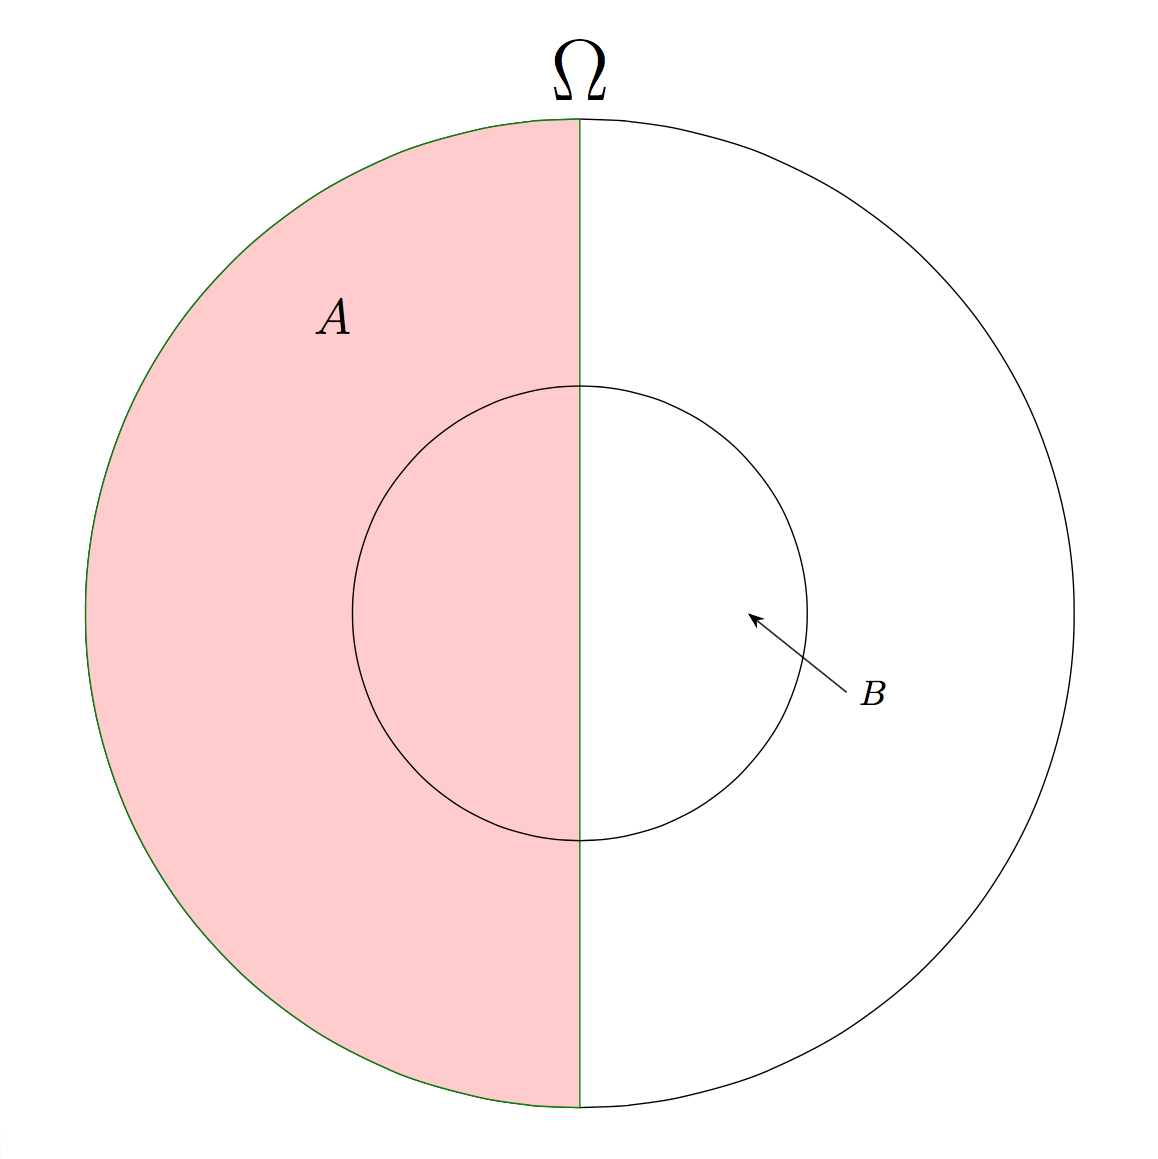
\includegraphics[width=6cm]{image/1.png}
    \vspace{0.25cm}
\end{Figure}

这里$B$是内圆,而$A$是红色的右半大圆,我们注意到,这两者占有全集$\Omega$的比例,与其各自在对方中的比例是相同的。例如,$B$在$\Omega$中,是半径较小的圆在一个半径较大的圆中,而另外一方面,$B$在$A$中,是半径较小的半圆在一个半径较大的半圆中。而类似的,$A$在$\Omega$中是一半,同时,$A$在$B$中也恰好是一半,这就形象的表现了条件概率与原概率相同的特点。

独立性的概念也可以推广到三个事件,设$A,B,C$是三个事件,若
\begin{Equation}
    \qquad\qquad
    P(AB)=P(A)P(B)\qquad
    P(BC)=P(B)P(C)\qquad
    P(CA)=P(C)P(A)
    \qquad\qquad
\end{Equation}
且
\begin{Equation}
    P(ABC)=P(A)P(B)P(C)
\end{Equation}
那就称$A,B,C$是独立的,由此亦可以推广至$n$个事件独立。